\section{Metrics for investigating feedback}
\label{sec:feedbackmetrics}

Feedback is a complex process that affects almost every possible metric that a
cosmological simulation can output. From the stellar mass function, to galaxy
sizes, all the way through to the density profiles of galaxies
\citep{BenitezLlambay2018}, feedback changes everything. It is concerning,
then, that there is no systematic way to study the effects of feedback on all
baryonic matter.

One reason that it is so difficult to investigate solely the feedback is that
it is impossible to tag all particles that have been involved in a given
feedback event. For a given feedback event, only a few particles are directly
involved (either by being kicked or having energy injected). However, these
particles will then go on to interact strongly with neighbouring gas
particles, which remain untagged. For example, in a traditional kinetic
feedback model, a handful of particles are kicked to high velocity which will
then go on to propagate high mach-number shockwaves throughout the ISM. Only
the initial particle is tagged as being invovled in that feedback event, even
though many more particles will be blown out of the potential well.

Thus the way to investigate feedback is to run one full model, and then
another with some features taken out by hand. This is at odds with the
minimisation procedure that many sub-grid models go through; many are
calibrated to the $z=0$ SMF, which will of course change should some feedback
mechanism be missing (and hence should be re-calibrated). These tests, then,
where the claim is usually that the SMF (or some other complex metric) cannot
be achieved without a certain feedback pathway, are invalid; by changing the
sub-grid parameters often the same result is reproducible.

A more direct metric to measure the effects of feedback is required, that is
independent of cosmology and astrophysics. Feedback is designed, in essence,
to spread particles out. Measuring spread is difficult in any simulation, but
particularly in one that uses Lagrangian methods; it should be completley
independent of rest frame to respect that nature. The spread measure proposed
here is based on neighbour finding in the initial and final conditions:

\begin{enumerate}
	\item For every particle $i$ in the initial conditions, find the nearest
		  dark matter neighbour $j$.
	\item In the final conditions, match all remaining baryonic particles
	      with their initial conditions progenitor (in this case, stars are
	      matched with their gas progenitor).
	\item In the final conditions, find the distance $r_{ij}$, i.e. the
	      distance between the original neighbours.
\end{enumerate}

\begin{figure*}
    \centering
    \includegraphics[width=\textwidth]{figures/distance_figure.pdf}
    \caption{The large-scale structure of the 50 Mpc reference model is shown.
    The background gray colour-map shows the projected column density of the
    gas in the simulation. Over-plotted is 1/250th of all gas particles
    in the simulation, coloured and sized by their distance travelled
    according to the metric below. Note how the low-distance particles
    are those that are trapped in the potential wells of the galaxies
    and clusters present in the simulations, with the particles that
    have travelled farther compared to their dark matter counterpart
    residing, in general, outside of any bound system.}
    \label{fig:feedbackpic}
\end{figure*}

A visualisation of this method is shown in Figure \ref{fig:feedbackpic}.
This method is completly independent of rest frame and can also be repeated
for the non-baryonic matter to see the effects of gravitational dynamics. In
experimenting with this metric, it appears that simply taking the base
distance for the nearest neighbour gives nearly equivalent results to taking
the median or mean distance over a number of closest neighbours, and so here
the more simple single distance measure is quoted.

\begin{figure}
	\centering
    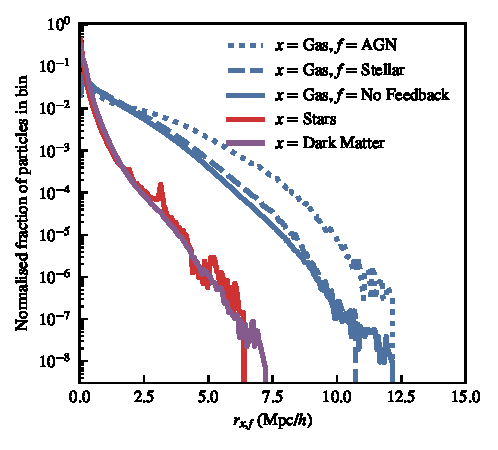
\includegraphics{generated_figures/m50n512s49/neighbour_analysis_feedback_histogram.pdf}
    \caption{
        The (normalised) distribution of distances for all particles $i$ to
        the nearest neighbour $j$ in the initial conditions, split by particle
        type. This is shown for the $z=0$ particle distribution in the
        reference model. Splitting the particles by those that have been
        involved in feedback events in this figure shows that the further
        out a particle has been blown the more likely it is to have been
        directly involved in a feedback event.
    }
    \label{fig:feedbackdistance}
\end{figure}

In Figure \ref{fig:feedbackdistance} the distribution of distances in the
reference model is shown. Note how similar the stellar distribution is to the
dark matter distribution even though strong feedback is included; this shows
that the star particles are mainly affected by gravitational dynamics and 
are mainly formed from gas that is in the core of the halo and can only end up
distances of around $6 \hmpc{}$. This is expected, as it is about twice the virial
radius of the largest halo in the simulation; a pair of initially neighbouring
particles can end up on opposite sides of a given halo. The gas, on the
other hand, can be blown out to very large distances (over $12 \hmpc{}$).

\begin{figure}
    \centering
    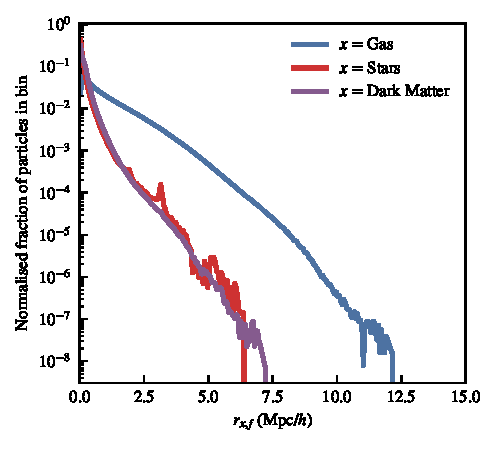
\includegraphics{generated_figures/m50n512s43nojet/neighbour_analysis_simple_histogram.pdf}
    \caption{
        The same metric as shown in Figure \ref{fig:feedbackdistance} but
        now for the \nojet{} model. Gas particles are still able to travel
        significantly further (note the 0.5-1 dex vertical offset relative)
        to the dark matter, but the long tail of particles out to $12 \hmpc{}$
        has been eliminated.
    }
    \label{fig:nojetdistance}
\end{figure}

Comparing to the \nojet{} run in Figure \ref{fig:nojetdistance}, it is clear
that the jets have a significant impact on the distances to which particles
are spread. Another interesting difference between these two plots is the
significant amount of entrained gas that they represent. When a particle is
directly involved in a feedback event (for example being blown out of an AGN
jet), they are tagged. However, the difference between these two plots shows
that the majority of gas that is blown out by such an event never directly
interacts with an AGN. This poses problems for analysis piplines that trust
that a reasonable proportion of gas that is involved in a given event is
correctly tagged.

These results show that gaseous and stellar matter can be transferred out
to significantly further (by $z=0$) than is assumed by typical zoom-in simulation
suites. For example, the Latte \citep{Wetzel2016} suite uses an exclusion region
for high resolution particles of around $1.5 \hmpc{}$. Whilst they do not find
contamination (possibly due to refinement criteria) of low-resolution particles
into the high-resolution region, the above metrics suggest that perhaps this is
a more numerical, rather than physical, effect; low resolution particles are
not present due to a lack of sub-grid physics in the unrefined region
